\documentclass[a4paper,12pt]{article}
\usepackage{cmap}					% поиск в PDF
\usepackage{mathtext} 				% русские буквы в формулах
\usepackage[T2A]{fontenc}			% кодировка
\usepackage[utf8]{inputenc}			% кодировка исходного текста
\usepackage[english,russian]{babel}	% локализация и переносы
\usepackage{indentfirst}
\frenchspacing

\usepackage{amsmath,amsfonts,amssymb,amsthm,mathtools} % AMS
\usepackage{amssymb,amsmath}
\usepackage{icomma} % "Умная" запятая: $0,2$ --- число, $0, 2$ --- перечисление

%% Номера формул
%\mathtoolsset{showonlyrefs=true} % Показывать номера только у тех формул, на которые есть \eqref{} в тексте.
%\usepackage{leqno} % Нумерация формул слева

%% Свои команды


%% Перенос знаков в формулах (по Львовскому)
\newcommand*{\hm}[1]{#1\nobreak\discretionary{}
	{\hbox{$\mathsurround=0pt #1$}}{}}

%%% Работа с картинками
\usepackage{graphicx}  % Для вставки рисунков
\graphicspath{{images/}{images2/}}  % папки с картинками
\setlength\fboxsep{3pt} % Отступ рамки \fbox{} от рисунка
%\setlength\fboxrule{1pt} % Толщина линий рамки \fbox{}
\usepackage{wrapfig} % Обтекание рисунков текстом

%%% Работа с таблицами
\usepackage{array,tabularx,tabulary,booktabs} % Дополнительная работа с таблицами
\usepackage{longtable}  % Длинные таблицы
\usepackage{multirow} % Слияние строк в таблице

%%% Теоремы
\theoremstyle{plain} % Это стиль по умолчанию, его можно не переопределять.
\newtheorem{theorem}{Теорема}[section]
\newtheorem{proposition}[theorem]{Утверждение}

\theoremstyle{definition} % "Определение"
\newtheorem{corollary}{Следствие}[theorem]
\newtheorem{problem}{Задача}[section]

\theoremstyle{remark} % "Примечание"
\newtheorem*{nonum}{Решение}

%%% Программирование
\usepackage{etoolbox} % логические операторы

%%% Страница
\usepackage{extsizes} % Возможность сделать 14-й шрифт
\usepackage{geometry} % Простой способ задавать поля
\geometry{top=10mm}
\geometry{bottom=15mm}
\geometry{left=10mm}
\geometry{right=10mm}

\usepackage{fancyhdr} % Колонтитулы
%	\pagestyle{fancy}
%\renewcommand{\headrulewidth}{0pt}  % Толщина линейки, отчеркивающей верхний колонтитул
% 	\lfoot{Нижний левый}
% 	\rfoot{Нижний правый}
% 	\rhead{Верхний правый}
% 	\chead{Верхний в центре}
% 	\lhead{Верхний левый}
%	\cfoot{Нижний в центре} % По умолчанию здесь номер страницы

\usepackage{setspace} % Интерлиньяж
\onehalfspacing % Интерлиньяж 1.5
%\doublespacing % Интерлиньяж 2
%\singlespacing % Интерлиньяж 1

\usepackage{lastpage} % Узнать, сколько всего страниц в документе.

\usepackage{soul} % Модификаторы начертания

\usepackage{hyperref}
\usepackage[usenames,dvipsnames,svgnames,table,rgb]{xcolor}
\hypersetup{				% Гиперссылки
	unicode=true,           % русские буквы в раздела PDF
	pdftitle={Заголовок},   % Заголовок
	pdfauthor={Автор},      % Автор
	pdfsubject={Тема},      % Тема
	pdfcreator={Создатель}, % Создатель
	pdfproducer={Производитель}, % Производитель
	pdfkeywords={keyword1} {key2} {key3}, % Ключевые слова
	colorlinks=true,       	% false: ссылки в рамках; true: цветные ссылки
	linkcolor=black,          % внутренние ссылки
	citecolor=black,        % на библиографию
	filecolor=magenta,      % на файлы
	urlcolor=cyan           % на URL
}

\usepackage{csquotes} % Еще инструменты для ссылок
\renewcommand{\labelitemi}{$\color{blue}{\bullet}$}
\renewcommand{\phi}{\varphi}
\renewcommand{\epsilon}{\varepsilon}
\usepackage[backend=biber,bibencoding=utf8,sorting=nyt,maxcitenames=2,style=apa]{biblatex}

\usepackage{multicol} % Несколько колонок
\newcolumntype{Y}{>{\centering\arraybackslash}X}

\usepackage{tikz} % Работа с графикой
\usepackage{pgfplots}
\usepackage{pgfplotstable}
\usepackage{caption}
\captionsetup{labelsep=period}
\usepackage{color, colortbl}
\usepackage[dvipsnames]{xcolor}
\usepackage[arrowdel]{physics}

\author{Елизавета Илюхина, Б07-301}
\title{3.7.1 Скин-эффект}
\date{}

\begin{document}
	\maketitle
	\paragraph{Цель работы:}  Исследование проникновения переменного магнитного поля в медный полый цилиндр
		\paragraph{В работе используются:} генератор звуковой частоты, соленоид, намотанный на полый цилиндрический каркас из диэлектрика, медный экран в виде трубки, измерительная катушка, амперметр, вольтметр, осциллограф.
		
	\section{Теоретические сведения}
	\subsection{Скин-эффект для полупространства}
		\begin{wrapfigure}{l}{0.3\textwidth}
	\begin{center}
			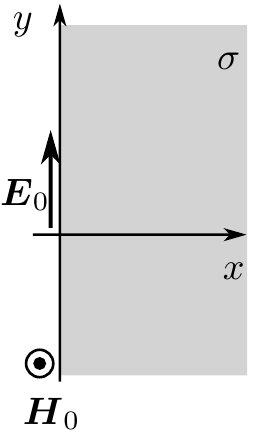
\includegraphics[width=0.28\textwidth]{poluprostranstvo}
		\end{center}
	\caption{Скин-эффект в полупространстве}\label{fig:poluprostranstvo}
	\end{wrapfigure}
	
	Рассмотрим квазистационарное поле внутри проводящей среды в простейшем плоском случае.
	Пусть вектор $\vb*{E}$ направлен всюду вдоль оси $y$ и зависит только от координаты $x$, т. е. ${E_x} = {E_z} \equiv 0$, $E_y=E_y(x,t)$.
	В квазистационарном приближении 
	\begin{equation*}
		\grad \times \vb*{H} = \sigma \vb*{E}
	\end{equation*}
	
	Преобразуя это уравнение, можно получить уравнение, схожее с уравнением диффузии:
	\begin{equation}
		\grad^2\vb*{H}=\sigma\mu\mu_0 \frac{\partial \vb*{H}}{\partial t}\label{eq:laplacian_H}
	\end{equation}
	Точно такое же уравнение имеет место и для вектора $E:$
	\begin{equation}
		\grad^2\vb*{E}=\sigma\mu\mu_0 \frac{\partial \vb*{E}}{\partial t}\label{eq:diffusion}
	\end{equation}
	
	Подставляем в (\ref{eq:diffusion}) наше электрическое поле $E_y=E_y(x,t)$
	\begin{equation}
		\frac{\partial^2 E_y}{\partial x^2} = \sigma\mu\mu_0\frac{\partial E_y}{\partial t}
		\label{eq:diffusion_chastni}
	\end{equation}
	Если $E_y(0,t)=E_0 e^{i\omega t}$ то решением (\ref{eq:diffusion_chastni}) будет функция вида
	\begin{equation}
		E_y(x,t)=E_0 e^{-x/\delta} e^{i(\omega t - x/\delta)}
		\label{eq:skin_effect_poluprostranstvo}
	\end{equation}
	где
	\begin{equation}
		\delta = \sqrt{\frac{2}{\omega\sigma\mu\mu_0}}
		\label{eq:delta}
	\end{equation}
	
	\subsection{Скин-эффект в тонком полом цилиндре}

		\begin{wrapfigure}{r}{4.5cm}
		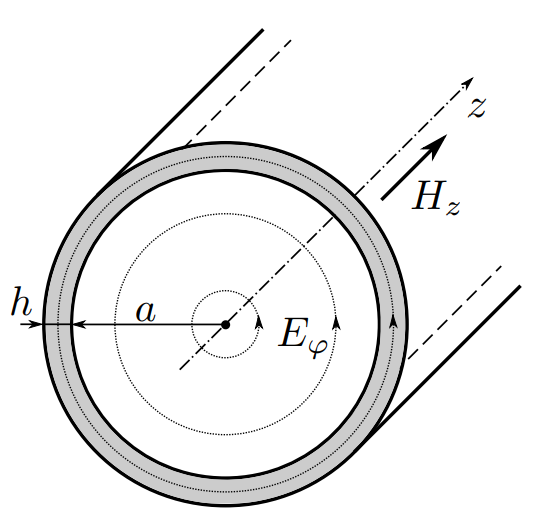
\includegraphics[width=5cm]{cylinder.png}
		\caption{Электрическое и магнитное поля в тонкостенном цилиндре}
		\label{pic:2}
	\end{wrapfigure}
	\indent Пусть цилиндр достаточно длинный, так что в нём можно пренебречь краевыми эффектами. В этом приближении магнитное поле $\vb*{H}$ всюду направлено по оси системы (ось $z$, а вихревое электрическое поле $\vb*{B}$ будет всюду перпендикулярно радиусу, то есть линии поля образуют соосные окружности (рис. 1). Все величины будем считать колеблющимися по гармоническому закону с некоторой частотой $\omega$ задаваемой частотой колебания тока в соленоиде. Тогда для ненулевых компонент поля можно записать
	\begin{equation*}
		H_z = H(r) e^{i \omega t}, \qquad E_{\varphi} = E(r) e^{i \omega t},
	\end{equation*}
	где $H(r)$ и $E(r)$ - комплексные амплитуды колебаний соответствующих полей, зависящие только от расстояния $r$ до оси системы. Заметим, что на границе цилиндра должны быть непрерывны касательные к поверхности компоненты как $\vb*{E}$, так и $\vb*{B}$, поэтому функции $H(r)$ и $E(r)$ непрерывны во всей исследуемой области.\\
	\indent Пусть длинный полый цилиндр имеет радиус $a$ и толщину стенки $h << a$. Последнее условие позволяет для описания поля внутри стенки ограничиться одномерным приближением. При этом для полного решения задачи необходимо вычислить и распределение поля внутри цилиндра.\\
	\indent Поскольку внутри цилиндра ток отсутствует, магнитное поле там является однородным: $H_z (r, t) = H_1 e^{i \omega t}$, где $H_1 = const$ - амплитуда поля на внутренней поверхности цилиндра. Для нахождения вихревого электрического поля
	воспользуемся законом электромагнитной индукции в интегральной форме:
	\begin{equation*}
		E_{\varphi} \cdot 2 \pi r = - \mu_0 \pi r^2 \cdot \frac{dH_z}{dt} \longrightarrow E(r) = -\frac{1}{2} \mu_0 r \cdot i \omega H_1.
	\end{equation*}
	\indent Отсюда получим \textbf{связь амплитуд колебаний электрического и магнитного полей} на внутренней ($r = a$) границе цилиндра:
	\begin{equation}\label{eq1}
		E_1 = -\frac{1}{2} i \omega a \mu_0 H_1.
	\end{equation}
	\indent Соотношение (\ref{eq1}) используем далее как дополнительное граничное условие для задачи о распределении поля внутри стенки.
	
	\begin{wrapfigure}{l}{5.5cm}
		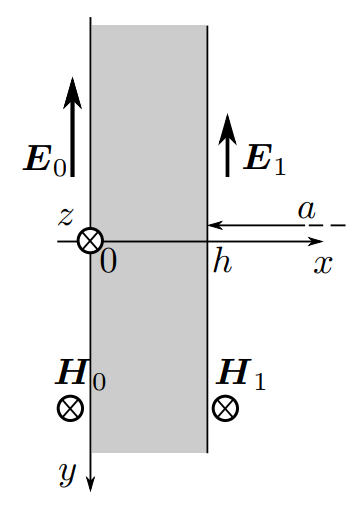
\includegraphics[width=4.5cm]{wall.png}
		\caption{Поле в стенке цилиндра}
		\label{pic:2}
	\end{wrapfigure}
	
	\indent Поле внутри тонкой стенки цилиндра («экрана») описывается уравнением скин-эффекта (уравнением диффузии поля) в плоской геометрии. Поместим начало отсчёта на внешнюю поверхность цилиндра и направим ось $x$ к оси системы, и запишем дифференциальное уравнение для комплексной амплитуды магнитного поля:
	\begin{equation}\label{eq2}
		\frac{d^2H}{dx^2} = i \omega \sigma \mu_0 H.
	\end{equation}
	(для медного цилиндра можно положить $\mu \approx 1$).\\
	\indent Граничные условия для (\ref{eq2}) зададим как:
	\begin{equation}\label{eq3}
		H(0) = H_0, \qquad H(h) = H_1.
	\end{equation}
	Здесь $H_0$ — амплитуда колебаний магнитного поля на внешней границе цилиндра. Её значение определяется только током в обмотке соленоида, и совпадает с полем внутри соленоида в отсутствие цилиндра. Величина $H_1$ также поддаётся непосредственному измерению — это амплитудa колебаний однородного поля внутри цилиндра. Поля $H_0$ и $H_1$ не являются независимыми — они связаны соотношением (\ref{eq1}).\\
	\indent Решение (\ref{eq2}) ищем в виде
	\begin{equation}\label{eq4}
		H(x) = A e^{\alpha x} + B e^{-\alpha x},
	\end{equation}
	где $A$, $B$ - определяемые из граничных условий константы,
	\begin{equation}\label{eq5}
		\alpha = \sqrt{i \omega \sigma \mu_0} = \frac{1 + i}{\delta} = \frac{\sqrt{2}}{\delta} e^{i \pi/4}
	\end{equation}
	- один из корней уравнения (\ref{eq2}), а $\delta$ - глубина скин-слоя (глубина проникновения поля) 
	\begin{equation}\label{eqdelta}
		\delta = \sqrt{\frac{2}{\omega \sigma \mu_0}}
	\end{equation}
	- характеристическое расстояние, на котором амплитуда поля уменьшается в $e$ раз. Мы имеем дело в конечной областью в виде плоского слоя толщиной $h$, поэтому решение уравнения (\ref{eq2}) должно содержать оба корня.\\
	\indent Из первого условия (\ref{eq3}): $A + B = H_0$, что позволяет исключить $A$ из (\ref{eq4}):
	\begin{equation*}
		H(x) = H_0 e^{-\alpha x} + 2B \sh \alpha x.
	\end{equation*}
	\indent Выразим электрическое поле из закона Ампера. В одномерном случае\\
	
	\begin{equation*}
		E(x) = \frac{1}{\sigma} \frac{dH}{dx} = \frac{\alpha}{\sigma} (H_0 e^{-\alpha x + 2B \ch \alpha x}).
	\end{equation*}
	
	\indent Далее положим $x = h$, воспользуемся (\ref{eq1}), и, исключив константу $B$, получим после преобразований \textbf{связь между $H_0$ и $H_1$}:\\
	\begin{equation}\label{eq6}
		H_1 = \frac{H_0}{\ch (\alpha h) + \frac{1}{2} \alpha a \sh(\alpha h)}.
	\end{equation}
	\indent Рассмотрим \textbf{предельные случаи уравнения (\ref{eq6})}: \\
	\indent \textbf{1}. При \textit{малых частотах} толщина скин-слоя превосходит толщину цилиндра $\delta >> h$. Тогда $|\alpha h| << 1$, поэтому $\ch \alpha h \approx 1$, $\sh \alpha h \approx \alpha h$ и 
	\begin{equation}\label{eq7}
		H_1 \approx \frac{H_0}{1 + i \frac{ah}{\delta^2}}.
	\end{equation}
	\indent Заметим, что величина $ah/\delta^2$ в общем случае не мала, поскольку при $h << a$ возможна ситуация $h << \delta << a$. Отношение модулей амплитуд здесь будет равно
	\begin{equation}\label{eq8}
		\frac{|H_1|}{|H_0|} = \frac{1}{\sqrt{1 + (\frac{ah}{\delta^2})^2}} = \frac{1}{\sqrt{1 + \frac{1}{4}(ah \sigma \mu_0 \omega)^2}}.
	\end{equation}
	\indent При этом колебания $H_1$ отстают по фазе от $H_0$ на угол $\psi$, определяемый равенством 
	
	\begin{equation}\label{eqq}
		tg \psi = \frac{ah}{\delta^2}
	\end{equation}
	
	\indent \textbf{2}. При достаточно \textit{больших частотах} толщина скин-слоя станет меньше толщины стенки: $\delta << h$. Тогда $|\alpha h| >> 1$ и $|\alpha a| >> 1$, а также $\sh(\alpha h) \approx \ch(\alpha h) \approx \frac{1}{2} e^{\alpha h}$. Выражение (\ref{eq6}) с учетом (\ref{eq5}) переходит в 
	\begin{equation}\label{eq9}
		\frac{H_1}{H_0} = \frac{4}{\alpha a} e^{\alpha h} = \frac{2\sqrt{2} \delta}{a} e^{-\frac{h}{\delta} e^{-i (\frac{\pi}{4} + \frac{h}{\delta})}}.
	\end{equation}
	
	\begin{figure}[h]
		\centering
		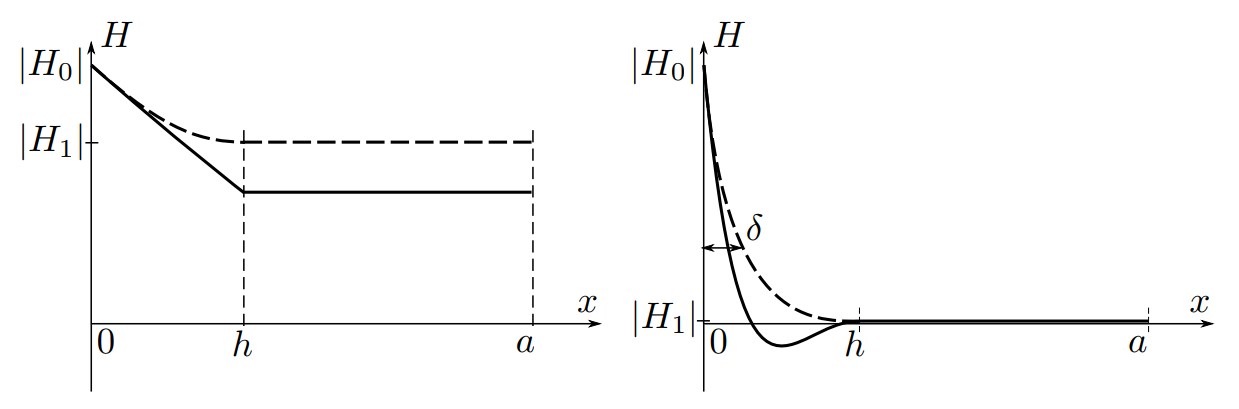
\includegraphics[width=0.9\linewidth]{fields.png}
		\caption{Распределение амплитуды колебаний магнитного поля (пунктир) и его мгновенного значения при некотором $t$ (сплошная) в зависимости от расстояния до внешней стенки цилиндра. Слева случай низких частот ($\delta >> h$), справа — скин-эффект при высоких частотах ($\delta << h$)}
		\label{fig:mpr}
	\end{figure}
	
	Как видно из формулы (\ref{eq9}), в этом пределе поле внутри цилиндра по модулю в $\frac{2\sqrt{2} \delta}{a} e^{-h/\delta}$ раз меньше, чем снаружи, и, кроме того, запаздывает по фазе на 
	
	\begin{equation}\label{eq10}
		\psi = \frac{\pi}{4} + \frac{h}{\delta} = \frac{\pi}{4} + h\sqrt{\frac{\omega \sigma \mu_0}{2}}.
	\end{equation}
	
	\indent На рис. 3 схематично изображено распределение магнитного поля от координаты в двух рассмотренных предельных случаях.\\

\subsection{Влияние скин-эффекта на индуктивность катушки}

Из-за скин-эффекта индуктивность соленоида с медным цилиндрическим экраном внутри будет зависеть от частоты тока. На высоких частотах магнитное поле не проникает внутрь соленоида (за экран), поэтому суммарный магнитный поток, пронизывающий катушку, уменьшается, и, соответственно, уменьшается и индуктивность. При низких частотах, когда толщина скин-слоя $\delta$ больше толщины медного экрана $h$, магнитное поле проникает внутрь катушки, однако его амплитуда падает \eqref{eq8} и возникает разность фаз между колебаниями поля за экраном и перед ним \eqref{eqq} Из-за этого также изменяется магнитный поток, а вместе с ним --- и индуктивность. 

Рассмотрим магнитный поток через катушку как сумму двух магнитных потоков: 1) пронизывающий область между катушкой и цилиндрическим экраном $\Phi_{out}$; 2) пронизывающий область за экраном $\Phi_{in}$:

\begin{equation}
	\Phi = \Phi_{out} + \Phi_{in} = H_0S_0 + H_1S_1 = LI,
\end{equation}
где $H_0, H_1$ --- \textit{мгновенные} значения магнитного поля внутри и снаружи цилиндра при данном токе $I$; $S_0, S_1$ --- площади внешней и внутренней областей соответственно.

Очевидно, что минимальная индуктивность будет в случае, когда $\Phi_{in} = 0$. При этом $L_{min}$ не зависит от частоты:

\begin{equation}
	L_{min} = \frac{\Phi_{out}}{I}.
\end{equation}
	
	Выразим поток магнитного поля сквозь внутреннюю область $\Phi_{in}$ через поток сквозь внешнюю $\Phi_{out}$ при произвольном переменном токе $I$:
	
	\begin{equation}
		\Phi_{in} = H_1S_1 = \frac{\Phi_{out} S_1}{nS_0},
	\end{equation}
	
	где коэффициент $n$, характеризующий ослабление поля за экраном, равен:
	
	\begin{equation}
		n = \frac{H_0}{H_1} = \frac{|H_0|}{|H_1|} \frac{1}{\cos \psi}.
	\end{equation}
	
	Максимальная индуктивность катушки достигается при максимальном потоке поля во внутренней области:
	\begin{equation}
		\Phi_{max} = \Phi_{in} + \Phi_{out} = H_0(S_0 +S_1) = L_{max}I,
	\end{equation}
	откуда получаем отношение площадей областей:
	\begin{equation}
		\frac{S_1}{S_0} = \frac{L_{max} - L_{min}}{L_{min}}.
	\end{equation}
	
	Суммируя все вышенаписанное, получаем индуктивность катушки:
	\begin{equation}
		L =L_{min} + \frac{L_{max} - L_{min}}{n}.
	\end{equation}
	
	Используя формулы \eqref{eq8}, \eqref{eqq}, \eqref{eq:delta}, окончательно получаем зависимость индуктивности катушки от частоты:
	\begin{equation} \label{eql}
		 \frac{L_{max} - L}{L- L_{min}} = (\pi ah\mu_0 \sigma \nu)^2.
	\end{equation}
	
	Данная зависимость может быть аппроксимирована прямой, по углу наклона которой можно найти проводимость.
	\section{Экспериментальная установка}
	\indent Схема экспериментальной установки для исследования проникновения переменного магнитного поля в медный полый цилиндр изображена на рис. 4. Переменное магнитное поле создаётся с помощью соленоида, намотанного на полый цилиндрический каркас 1 из поливинилхлорида, который подключается к генератору звуковой частоты. Внутри соленоида расположен медный цилиндрический экран 2. Для измерения магнитного поля внутри экрана используется измерительная катушка 3.\\
	\indent Необходимые параметры соленоида, экрана и измерительной катушки
	указаны на установке: \\
	\indent Действующее значение переменного тока в цепи соленоида измеряется амперметром $A$, а действующее значение напряжения на измерительной катушке измеряет вольтметр $V$. Для измерения сдвига фаз между током в цепи соленоида и напряжением на измерительной катушке используется двухканальный осциллограф. На вход одного канала подаётся напряжение с резистора $R$, которое пропорционально току, а на вход второго канала — напряжение с измерительной катушки.\\
	\begin{figure}[h]
		\centering
		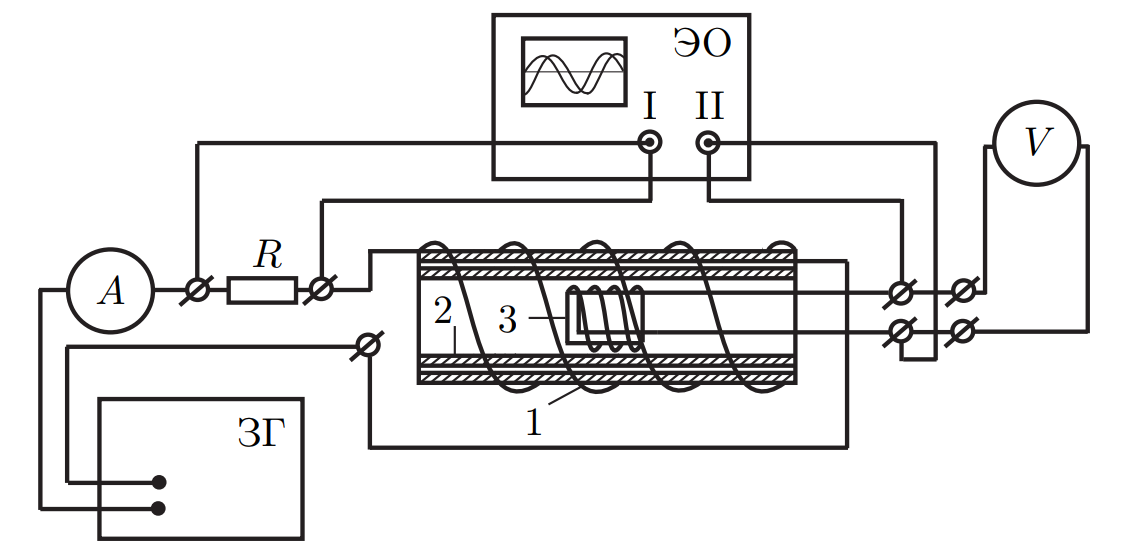
\includegraphics[width=0.75\linewidth]{ust.png}
		\caption{Экспериментальная установка для изучения скин-эффекта}
	\label{fig:mpr}
	\end{figure}
	
	\subsection{Измерение отношения амплитуд магнитного поля внутри и вне экрана}
	
	\indent С помощью вольтметра $V$ измеряется действующее значение ЭДС индукции, которая возникает в измерительной катушке, находящейся в переменном магнитном поле $H_1 e^{i \omega t}$. Комплексная амплитуда ЭДС индукции в измерительной катушке равна 
	\begin{equation*}
		U = -SN \frac{dB_1 (t)}{dt} = -i \omega \mu_0 SN H_1 e^{i \omega t},
	\end{equation*}
	где $SN$ - произведение площади витка на число витков измерительной катушки. Показания вольтметра, измеряющего это напряжение:
	\begin{equation*}
		U = \frac{SN \omega}{\sqrt{2}} \mu_0 |H_1|.
	\end{equation*}
	\indent Видно, что модуль амплитуды магнитного поля внутри экрана $|H_1|$ пропорционален $U$ и обратно пропорционален частоте сигнала $\nu = \omega/2\pi$:
	\begin{equation*}
		|H_1| \propto \frac{U}{\nu}.
	\end{equation*}
	\indent При этом поле вне экрана $|H_0|$ пропорционально току $I$ в цепи соленоида, измеряемому амперметром $A$:
	\begin{equation}
		|H_0| \propto I.
	\end{equation}
	Следовательно, 
	\begin{equation} \label{eq11}
		\frac{|H_1|}{|H_0|} = const \cdot \frac{U}{\nu I}.
	\end{equation}
	\indent Таким образом, отношение амплитуд магнитных полей снаружи и вне экрана (коэффициент ослабления) может быть измерено по отношению $U/\nu I$ при разных частотах. Неизвестная константа в соотношении (\ref{eq11}) может быть определена по измерениям при малых частотах $\nu$ $\longrightarrow$ 0, когда, согласно (\ref{eq8}) $|H_1|/|H_0|$ $\longrightarrow$ 1.\\
	
	\indent ЭДС индукции в измерительной катушке 
	\begin{equation*}
		\mathcal{E}_i=-SN\dfrac{dB_{0c}(t)}{dt}=-\mu_0 SN \dfrac{dH_{1}(t)}{dt} = -i \mu_0 SN\omega H_{1} e^{i \omega t},
	\end{equation*}
	где $SN$ - произведение площади витка на количество витков измерительной катушки. Обозначим показания вольтметра $V$ через $U_{\text{к}}$, тогда 
	\begin{equation*}
		U_{\text{к}} = \dfrac{mu_0SN\omega}{\sqrt{2}}|H_{1}|.
	\end{equation*}
	Из этого соотношения следует, что абсолютная величина амплитуды магнитного поля внутри экрана: \\
	$$|H_{1}| \sim \dfrac{U_{\text{к}}}{\omega} \sim \dfrac{U_{\text{к}}}{\nu},$$ где $\nu$ частота генератора. Но поле внутри экрана пропорционально полю вне экрана $H_0$, а $H_0\sim I_A$, где $I_A$ - показания амперметра А в цепи соленоида. Следовательно, амплитуда поля внутри экрана, приведенная к единичному току через соленоид, $$|H_{1}| \sim \dfrac{U_{\text{к}}}{\nu I_A}.$$ Обозначим величину, пропорциональную $|H_{1}|$, через $\xi_{1}$:
	
	\begin{equation}
		\xi_{1} = \dfrac{U_{\text{к}}}{\nu I_A}.
	\end{equation}
	Нам теперь необходимо найти амплитуду поля вне экрана при том же единичном токе через соленоид. Для этого воспользуемся соотношением (27). Проведя измерения $\xi_{1}$ в диапазоне самых малых частот, мы построим график зависимости $\xi_{1}$ от $\nu^2$. Согласно (27) эта зависимость имеет вид прямой. Экстраполируя ее к $f=0$, мы получим $\xi_{0c}(0) = \xi_0$, которая пропорциональна амплитуде поля вне экрана при единичном токе через соленоид. Отношение амплитуд магнитного поля внутри экрана и вне при фиксированно частоте $f$ будет равно 
	\begin{equation}\label{last}
		\dfrac{|H_{1}|}{|H_0|} = \dfrac{\xi_{1}(\nu)}{\xi_0} = \dfrac{U_{\text{к}}}{\nu I_A\xi_0}.
	\end{equation}
	Такой способ измерения коэффициента ослабления магнитного поля проводящим экраном не требует поддерживать постоянный ток через соленоид при измерении частотной зависимости этого коэффициента.
	
	\subsection{Определение проводимости материала экрана}
	
	\indent В установке в качестве экрана используется медная труба промышленного производства. Технология изготовления труб оказывает заметное влияние на электропроводимость. Из-за наличия примесей проводимость меди нашей трубы отличается от табличного значения (в меньшую сторону). Для определения $\sigma$ нашего экрана предлагается использовать частотную зависимость (\ref{eq10}) фазового сдвига между магнитными полями внутри и вне экрана при высоких частотах. \\
	\indent Как видно из выражения (\ref{eq10}), в области больших частот $\omega >> 1/(h^2 \sigma \mu_0)$ зависимость $\psi (\sqrt{\omega})$ аппроксимируется прямой, проходящей через точку $\psi (0) = \pi/4$. По наклону этой прямой можно вычислить проводимость материала экрана.\\
	\indent Заметим, что на схеме, изображённой на рис. 4, на входной канал II осциллографа подаётся сигнал с измерительной катушки, который пропорционален не полю внутри экрана, а его производной по времени, а это означает, что появляется дополнительный сдвиг по фазе на $\pi/2$. Поэтому измеренный по экрану осциллографа сдвиг по фазе между двумя синусоидами будет на $\pi/2$ больше фазового сдвига между магнитными полями вне и внутри экрана.
	
	\section{Ход работы}
	
	По известным параметрам установки $2a = 45$ мм, $h=1.5$ мм, приняв проводимость порядка
	$\sigma \sim 5\cdot 10^7$ См/м, рассчитаем частоту, при которой
	глубина проникновения равна толщине стенок цилиндра $\nu_h = 2245$ Гц.
	
	\subsection{Измерение проводимости через измерение амплитуд в области низких частот}
	
Установим начальную частоту сигнала генератора $\sim 0,01 \nu_h \approx 22,45$ Гц. В области низких частот ($0,01 \nu_h - 0,05 \nu_h$) получим зависимость отношения $\xi = u/\nu I$ от частоты $\nu$. Согласно \eqref{last} величина $\xi$ прямо пропорциональна коэффициенту ослабления магнитного поля внутри экрана относительно поля снаружи:

\begin{equation*}
	\xi = \xi_0 \frac{|H_1|}{|H_0|}.
\end{equation*}
	
	При этом $\sigma_{\xi} = \xi \sqrt{\left(\frac{\sigma_U}{U}\right)^2 + \left(\frac{\sigma_I}{I}\right)^2}$.
	
	Построим график в координатах $1/\xi^2 = f(\nu^2)$. Экстраполируя зависимость к $\nu = 0$, где $|H_1|/|H_0| = 1$ найдем коэффициент пропорциональности $\xi_0$ между $\xi$ и ослаблением магнитного поля:
	
		\begin{equation}
		\xi_0 = 14,52 \pm 0,01 \frac{\text{Ом}}{\text{кГц}}. \ \ \ (0,07 \%)
	\end{equation}
	
		
	По угловому коэффициенту рассчитаем проводимость меди:
	
	\begin{equation*}
		\frac{\xi^2}{\xi_0^2} = \frac{1}{1 + \cfrac{1}{4}(ah\sigma \mu_0 \omega)^2} \longrightarrow \frac{\xi^2_0}{\xi^2} = 1 + \pi^2 a^2 h^2 \sigma^2 \mu_0^2 \nu^2,
	\end{equation*}
	
	\begin{equation}
		k _1 = 0,164 \pm 0,003 \frac{1}{\text{Ом}^2} = \frac{\pi^2 a^2 h^2 \sigma^2 \mu_0^2}{\xi_0^2} \longrightarrow \sigma = (4,40 \pm 0,02) \cdot 10^7 \frac{\text{См}}{\text{м}}. \ \ \  (0,5\%)
	\end{equation}
	
	\includegraphics[width = 0.8\textwidth]{xi1}
	
		\begin{table}[h]
		\begin{tabularx}{\textwidth}{|c|Y|Y|Y|Y|Y|Y|Y|Y|}
			\hline
			\# & 1 & 2 & 3 & 4 & 5 & 6 & 7 & 8 \\
			\hline
			$\dfrac{1}{\xi^2}\cdot 10^{-3}, \frac{\text{Гц}^2 \text{А}^2}{\text{В}^2}$ & 4830,5&		4904&			5053&	5244,75&			5483,22&			5757,72&			6075,09&			6430,75 \\	\hline
			$\nu^2 \cdot 10^{-3}, \text{ Гц}^2$ & 504&			1134,34&			2016&			3150,6&			4536,02&			6174,8&			8064&			10207	 \\ \hline
			\hline
			\# & 9& 10 & 11 & 12 & 13 & 14 & 15 & 16 \\
			\hline
			$\dfrac{1}{\xi^2}\cdot 10^{-3}, \frac{\text{Гц}^2 \text{А}^2}{\text{В}^2}$ & 6831,65 & 			7272,45&			7714,86&			8787,5&			10027&			11432,8&			13003& \\	\hline
			$\nu^2 \cdot 10^{-3}, \text{ Гц}^2$ & 12600& 15247&			18144&			24696&			32256,2&			40824&			50400 &\\ \hline
			
				\end{tabularx}
		\label{tab:my-table1}
	\end{table}
	
	\subsection{Измерение проводимости через разность фаз при низких частотах}
	
	Будем исследовать зависимость величины   $\psi$  фазового сдвига  от частоты  $\nu$  при частотах в диапазоне $0,05 \nu_h - 0,5 \nu_h$. Учтем сдвиг фаз. 
	
			Согласно формуле \eqref{eqq}, при низких частотах поле $H_1$  отстает от поля $H_0$ на фазу:
	\begin{equation*}
		\tan \psi \approx \pi a h \sigma \mu_0 \nu  \ \ \ (\text{В нашем эксперименте } \mu = 1).
	\end{equation*}
	
	Коэффициент наклона прямой:
	\begin{equation}
		k_2 = (6,03 \pm 1,93) \cdot 10^{-3} \ c. \ \ \ (32 \%)
	\end{equation}
	
	Отсюда проводимость:
	
	\begin{equation}
		\sigma = \frac{k_2}{\pi a h \mu_0} = (4,51 \pm 1,44) \cdot 10^7  \frac{\text{См}}{\text{м}}. \ \ \ (32\%)
	\end{equation}
	
		\includegraphics[width = 0.8\textwidth]{psi1}
		
				\begin{table}[h]
			\begin{tabularx}{\textwidth}{|c|Y|Y|Y|Y|Y|Y|Y|Y|Y|}
				\hline
				\# & 1 & 2 & 3 & 4 & 5 & 6 & 7 & 8 & 9 \\
				\hline
			$	\tan\psi$& 0,867 &			0,921&			1&			1,254&			1,732&			1,556&			2,246&			3,406&			6,955	\\ \hline
			$\sigma_{\tan \psi}$ & 0,091&			0,112&			0,143&			0,193&			0,315&			0,311&			0,321&			0,649&			0,647 \\ \hline
				$\nu, \text{ Гц}$ &112,25&				134,7&				157,15&				179,6&				202,05&				224,5&				336,75&				449&				561,25	 \\ \hline
	
			\end{tabularx}
			\label{tab:my-table2}
		\end{table}
		
			\subsection{Измерение проводимости через разность фаз при высоких частотах}
			
				Теперь исследуем зависимость величины   $\psi$  фазового сдвига  от частоты  $\nu$  при частотах в диапазоне $0,5 \nu_h - 15 \nu_h$. Учтем сдвиг фаз. 
			
			Согласно формуле \eqref{eq10}, при $\delta << h $ разность фаз:
			
			\begin{equation*}
				\psi - \frac{\pi}{4} = h\sqrt{\pi \mu_0 \sigma \nu }
			\end{equation*}
		
		Построим график в координатах $(\psi - \frac{\pi}{4} ) = f(\sqrt{\nu})$. Через начало координат проведем прямую, которая будет касаться экспериментальной кривой при больших частотах.
		
		\begin{equation}
			k_3 = 0,678 \pm 0,068 \frac{1}{\sqrt{\text{кГц}}} \ \ \ (10\%)
		\end{equation}
		
		По наклону этой прямой вычислим проводимость:
		
		\begin{equation}
			\sigma = \frac{k_3^2}{h^2\pi \mu_0} = (5,16 \pm 1,03) \cdot 10^7 \frac{\text{См}}{\text{м}}. \ \ \  (20\%)
		\end{equation}
		
		
				\includegraphics[width = 0.8\textwidth]{pv}
				
								\begin{table}[h]
					\begin{tabularx}{\textwidth}{|c|Y|Y|Y||c|Y|Y|Y|}
						\hline
						\# & $\sqrt{\nu}, \ \sqrt{\text{кГц}}$  & $\psi - \cfrac{\pi}{4},$ рад. & $\sigma_{\psi},$ рад. &	\# & $\sqrt{\nu}, \ \sqrt{\text{кГц}}$  & $\psi - \cfrac{\pi}{4},$ рад. & $\sigma_{\psi},$ рад. \\ \hline
1& 0,335&	-0,071&	-0,00888& 18 &1,621	& 1,116	&0,11747 \\ \hline
2 &0,367&	-0,04&	-0,00571 & 19 &1,773&	1,178	&0,14725 \\ \hline
3 &0,396&	0&	0& 20& 1,895	&1,234&	1,234  \\ \hline
4 &0,424&	0,112&	0,02036 &21 &2,092&	1,357&	1,357 \\ \hline
5 &0,449&	0,262&	0,0524 &22 &2,272&	1,414	&0,5656 \\ \hline
6 &0,474&	0,214&	0,04756 &23& 2,462	&1,533&	0,6132 \\ \hline
7 &0,58	&0,367	&0,05646 &24& 2,68	&1,709&	0,6836 \\ \hline
8 &0,67	&0,5&	0,1 &25& 2,921	&1,907&	0,63567 \\ \hline
9 &0,749&	0,643&	0,06124& 26& 3,214&	2,132&	0,4264 \\ \hline
10& 0,821&	0,785&	0,08722& 27& 3,482&	2,281&	0,4562 \\ \hline
11 &0,886&	0,785&	0,09813& 28& 3,791&	2,531&	0,5062 \\ \hline
12 &0,948&	0,785&	0,11214 &29 &4,13&1	2,88&	0,576 \\ \hline
13 &1,005&	0,785&	0,13083& 30 &4,495&	3,202&	0,33705 \\ \hline
14 &1,059&	0,785&	0,07136 & 31& 4,901	&3,478&	0,38644 \\ \hline
15& 1,16&	0,951	&0,10011& 32 &5,319	&4,102&	0,45578 \\ \hline
16& 1,254&	0,982&	0,12275 &33 &5,803	&5,105&	3,40333 \\ \hline
17& 1,365	&1,027&	0,158& 34 &1,498&	1,071&	0,09736 \\ \hline
					\end{tabularx}
					\label{tab:my-table3}
				\end{table}
			
		\subsection{Измерение проводимости через изменение индуктивности}
		
		Соберем схему согласно рисунку:
		
								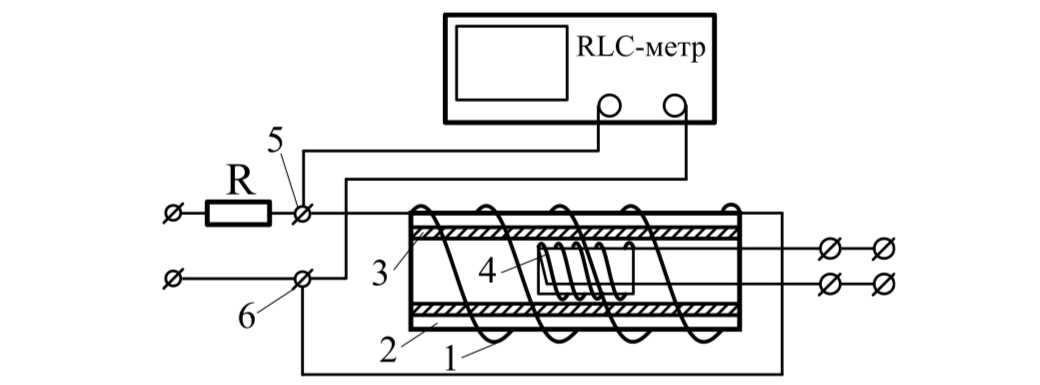
\includegraphics[width = 0.8\textwidth]{rlc}
								
		Снимем зависимость индуктивности катушки от частоты. Построим график и по нему определим максимальное и минимальное значения индуктивности.
		
		\begin{align}
			L_{min} &= 2,93 \text{ мГн} \\
			L_{max} &= 10,35  \text{ мГн}
		\end{align}
		
						\includegraphics[width = 0.8\textwidth]{lv}
						
									\begin{table}[h]
		\begin{tabularx}{\textwidth}{|c|Y|Y|Y|Y|Y|Y|Y|}
			\hline
		\# & 1 & 2 & 3 & 4 & 5 & 6 & 7\\ \hline
		$\nu,$ Гц & 40 & 150 & 200 & 250 & 300 & 400 & 500 \\ \hline
		$L,$ мГн & 10,35 & 7,44 & 6,32 & 5,5 &4,91 & 4,18 & 3,77 \\ \hline
		\# & 8 & 9 & 10 & 11 & 12 & 13 & 14 \\ \hline
		$\nu,$ Гц  & 600 & 800  & 1500 & 2000 & 2500 & 3000 & 4000 \\ \hline
		$L,$ мГн & 3,53 & 3,27 & 3,01& 2,97 & 2,95 & 2,94 & 2,93 \\ \hline
		\end{tabularx}
		\label{tab:my-table4}
	\end{table}					
						
Построим график $\frac{L_{max} - L}{L - L_{min}} = f(\nu^2)$. Из формулы \eqref{eql}  и коэффициента наклона мы можем						вычислить проводимость:

\begin{equation}
	k_4 = \pi^2 a^2 h^ 2 \mu_0^2 \sigma^2 = 32,76 \pm 0,22 \frac{1}{\text{кГц}^2} \ \ \ (1\%)
\end{equation}

Отсюда проводимость:

\begin{equation}
	\sigma = \frac{\sqrt{k_4}}{\pi a h \mu_0} = (4,28 \pm 0,02) \cdot 10^7  \frac{\text{См}}{\text{м}}. \ \ \  (0,5\%)
\end{equation}

						\includegraphics[width = 0.8\textwidth]{llv}
						
											\begin{table}[h]
			\begin{tabularx}{\textwidth}{|c|Y|Y|Y|Y|Y|Y|Y|Y|Y|}
				\hline
				\# & 1 & 2 & 3 & 4 & 5 & 6 & 7 & 8 & 9  \\ \hline
				$\nu^2, \text{ кГц}^2$ & 0,0016&				0,0225&				0,0625&				0,16&				0,25&				0,09&				0,36&				0,04&				0,64 \\ \hline
				$\dfrac{L_{max} - L}{L - L_{min}}$ & 0&				0,64595&				1,89425&				4,97438&				7,85383&				2,75707&				11,45665&				1,19063&				20,968\\ \hline

			\end{tabularx}
			\label{tab:my-table5}
		\end{table}	
		
		\section{Предварительные итоги}
		
		Мы измерили проводимость четырьмя способами. Сравним их между собой и с табличным значением. Для этого занесем все полученные результаты в таблицу.
													\begin{table}[h]
																\begin{center}
			\begin{tabularx}{0.7\textwidth}{|c|Y|Y|Y|}
				\hline
			Метод измерения & $\sigma,  10^7  \frac{\text{См}}{\text{м}}$ & $\sigma_{\sigma}, 10^7  \frac{\text{См}}{\text{м}}$ & $\epsilon_{\sigma}, \%$ \\ \hline
			Отношение амплитуд& 4,40 & 0,02 & 0,5 \\ \hline
			Разность фаз (низкие частоты)& 4,51 & 1,44 & 32 \\ \hline
			Разность фаз (высокие частоты)& 5,16 & 1,03 & 20 \\ \hline
			Индуктивность&4,28 & 0,02 & 0,5 \\ \hline
			Табличное&5,62 & - & - \\ \hline
			\end{tabularx}
							\end{center}
			\label{tab:my-table6}
		\end{table}	
		
		Полученные нами значения совпадают по порядку, но меньше табличного значения. Несовпадение может быть вызвано многими факторами, например наводкой поля в соединительных проводах и пренебрежением размерами медного цилиндра и соленоида. 
		
		Методы измерения через разность фаз дали высокие погрешности, потому что измерения делались на глаз на осциллографе, и цена деления там была достаточно большая относительно измеряемых величин, поэтому данные методы были наименее точными (32 \% и 20\%). Кроме того, при измерении на высоких частотах зависимость не является везде линейной, это тоже привносит свою неточность.
		
\section{Отношение полей }		
Построим экспериментальную зависимость $\frac{|H_1|}{H_0} (\ln{\nu})$, используя формулу (\ref{last}), а также две теоретические (для наибольшего и наименьшего из полученных значений $\sigma$) по формуле \eqref{eq6}. Таблицы вышли очень громоздкие, поэтому прикреплять их не буду.

						\includegraphics[width = 0.8\textwidth]{h1h0}
						
			Видим, что экспериментальные данные хорошо согласуются с теорией --- экспериментальная зависимость полностью лежит между теоретическими, практически совпадая с одной из них. Так как теоретические значения были рассчитаны с помощью программы на питоне, в связи с его численными методами вычисления тригонометрических функций, могла возникнуть систематическая погрешность, оценить которую я не могу.
			
\end{document}
